\documentclass[tikz,border=12pt]{standalone}
\usepackage[T1]{fontenc}
\usepackage{mathpazo}
\usepackage{amsmath,amssymb}
\usetikzlibrary{arrows.meta, positioning, calc, fit, decorations.pathreplacing}

\definecolor{stblue}{HTML}{7B97AD}
\definecolor{rwgold}{HTML}{B8995E}
\definecolor{sage}{HTML}{7A9A7E}
\definecolor{dkbrown}{HTML}{3D3530}
\definecolor{wmgray}{HTML}{7B7067}
\definecolor{cream}{HTML}{F9F6F0}
\definecolor{border}{HTML}{D4C9B8}
\definecolor{terracotta}{HTML}{C47A6A}
\definecolor{lavender}{HTML}{907EA0}

\begin{document}
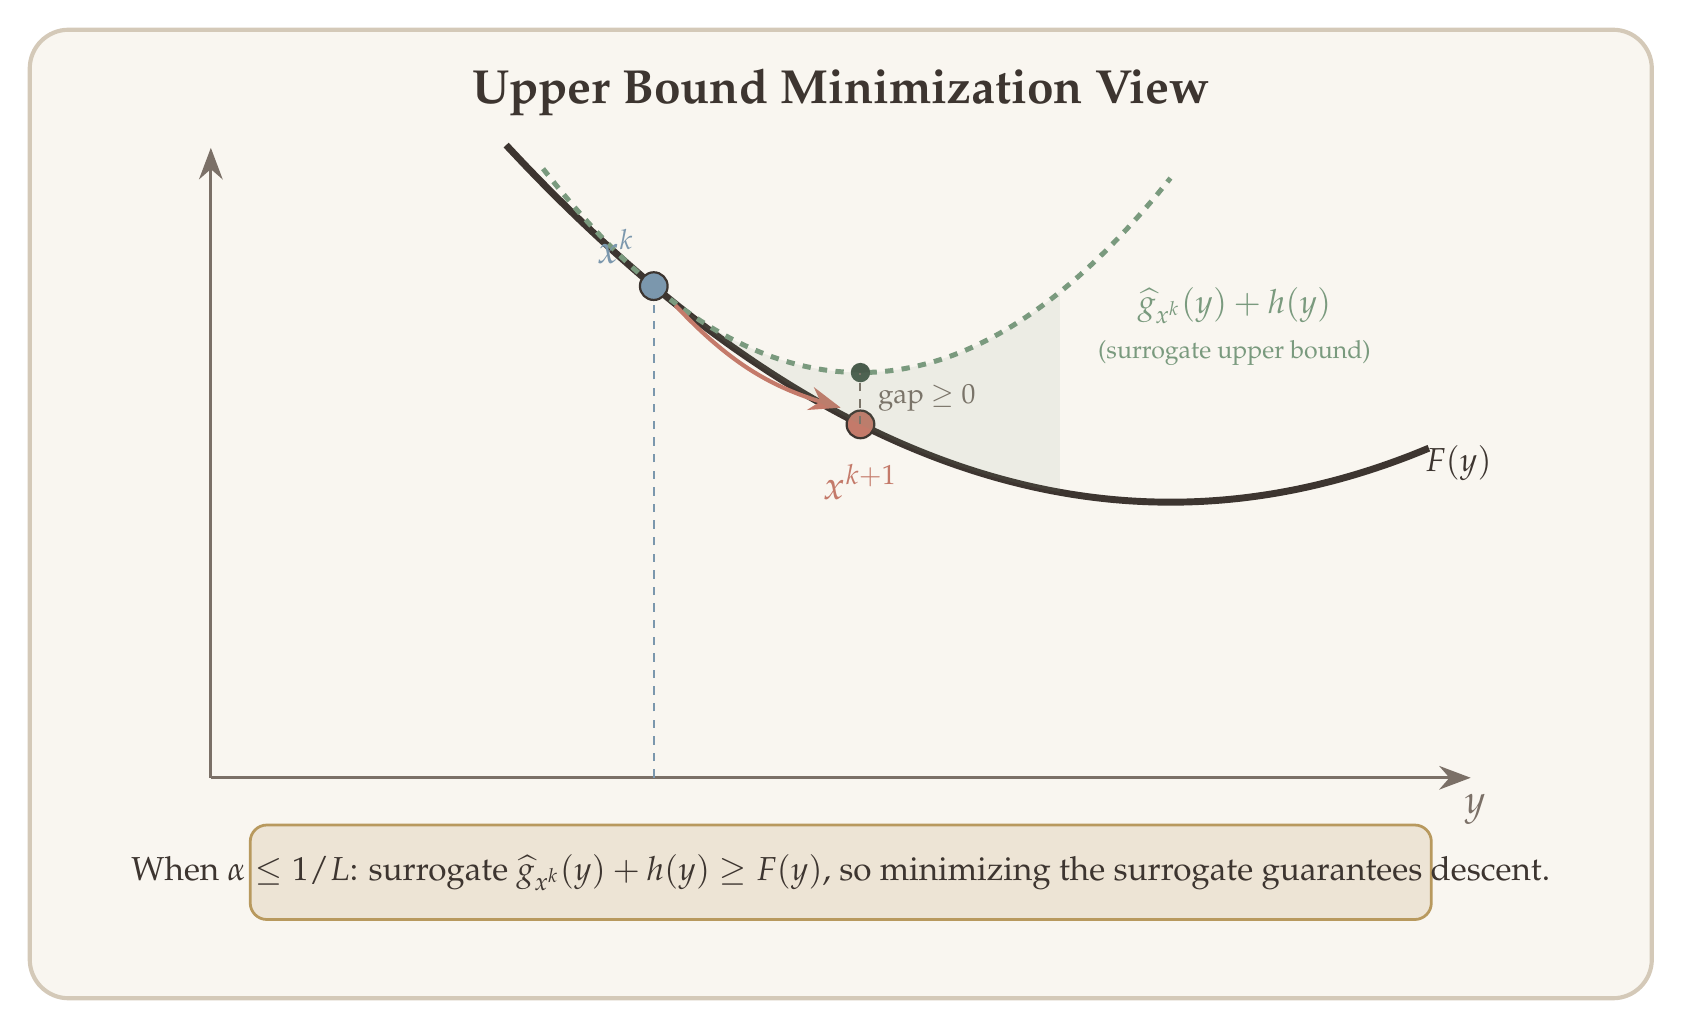
\begin{tikzpicture}[>={Stealth[length=4mm, width=3mm]}]

% Background
\fill[cream, rounded corners=14pt] (-0.8,-0.8) rectangle (19.8,11.5);
\draw[border, line width=1.5pt, rounded corners=14pt] (-0.8,-0.8) rectangle (19.8,11.5);

% Title
\node[text=dkbrown, font=\LARGE\bfseries] at (9.5,10.7) {Upper Bound Minimization View};

% Axes
\draw[wmgray, line width=1pt, ->] (1.5,2.0) -- (17.5,2.0);
\draw[wmgray, line width=1pt, ->] (1.5,2.0) -- (1.5,10.0);
\node[text=wmgray, font=\Large, right] at (17.3,1.6) {$y$};

% Coordinate system:
% y-axis (horizontal): canvas_x = 1.5 + y_val * 0.9375  (y_val from 0 to 17)
% F-axis (vertical):   canvas_y = 2.0 + F_val * 1.4      (F_val from 0 to ~5.5)

% F(y) = 0.04*(y - 13)^2 + 2.5   (convex quadratic, minimum at y=13, F(13)=2.5)
% Canvas: x = 1.5 + y*0.9375,  height = 2.0 + F*1.4

% Plot F(y) from y=2 to y=17
% Sample points:
% y=2:  F=7.34 -> (3.375, 12.276) -- too high, clip
% y=3:  F=6.5  -> (4.3125, 11.1)  -- too high
% y=4:  F=5.74 -> (5.25, 10.036)
% y=5:  F=5.06 -> (6.1875, 9.084)
% y=6:  F=4.46 -> (7.125, 8.244)
% y=7:  F=3.94 -> (8.0625, 7.516)
% y=8:  F=3.5  -> (9.0, 6.9)
% y=9:  F=3.14 -> (9.9375, 6.396)
% y=10: F=2.86 -> (10.875, 6.004)
% y=11: F=2.66 -> (11.8125, 5.724)
% y=12: F=2.54 -> (12.75, 5.556)
% y=13: F=2.5  -> (13.6875, 5.5)
% y=14: F=2.54 -> (14.625, 5.556)
% y=15: F=2.66 -> (15.5625, 5.724)
% y=16: F=2.86 -> (16.5, 6.004)

% F(y) curve (convex)
\draw[dkbrown, line width=2.5pt, smooth, samples=50, domain=4:16.5]
  plot ({1.5 + \x*0.9375}, {2.0 + (0.04*(\x-13)*(\x-13) + 2.5)*1.4});
\node[text=dkbrown, font=\large, right] at (16.8,6.0) {$F(y)$};

% x^k at y=6: F(6) = 0.04*49 + 2.5 = 4.46
% canvas: (7.125, 8.244)

% Surrogate: g_hat_x(y) = F(x^k) + F'(x^k)*(y - x^k) + (L/2)*(y - x^k)^2
% F'(y) = 0.08*(y-13), so F'(6) = 0.08*(-7) = -0.56
% Choose L = 0.16 (so L/2 = 0.08, matching true curvature would give exact bound)
% But we want surrogate > F, so pick L = 0.20 (L/2 = 0.10)
% g_hat(y) = 4.46 + (-0.56)*(y-6) + 0.10*(y-6)^2
%          = 4.46 - 0.56*y + 3.36 + 0.10*(y^2 - 12y + 36)
%          = 4.46 + 3.36 + 3.6 - 0.56y - 1.2y + 0.10*y^2
%          = 11.42 - 1.76y + 0.10*y^2
% Minimizer: y* = 1.76/(2*0.10) = 8.8
% g_hat(8.8) = 4.46 - 0.56*2.8 + 0.10*7.84 = 4.46 - 1.568 + 0.784 = 3.676
% F(8.8) = 0.04*(8.8-13)^2 + 2.5 = 0.04*17.64 + 2.5 = 3.2056
% Gap = 3.676 - 3.2056 = 0.47, good!
% Check at x^k: g_hat(6) = 4.46, F(6) = 4.46. Touches!
% Check at y=2: g_hat(2) = 11.42 - 3.52 + 0.4 = 8.3, F(2) = 7.34. Above!
% Check at y=14: g_hat(14) = 11.42 - 24.64 + 19.6 = 6.38, F(14) = 2.54. Above!

% Plot surrogate from y=4.5 to y=13
\draw[sage, line width=1.8pt, dashed, smooth, samples=50, domain=4.5:13]
  plot ({1.5 + \x*0.9375}, {2.0 + (4.46 - 0.56*(\x-6) + 0.10*(\x-6)*(\x-6))*1.4});
\node[text=sage, font=\large] at (14.5,8.0) {$\widehat{g}_{x^k}(y) + h(y)$};
\node[text=sage, font=\large] at (14.5,7.4) {\small (surrogate upper bound)};

% Mark x^k point on F(y)
\fill[stblue] (7.125,8.244) circle (5pt);
\draw[dkbrown, line width=0.8pt] (7.125,8.244) circle (5pt);
\node[text=stblue, font=\Large, above left] at (7.0,8.4) {$x^k$};

% Mark tangent point: surrogate touches F at x^k
% Both curves pass through (7.125, 8.244)

% x^{k+1} at y=8.8: F(8.8) = 3.2056 -> canvas (9.75, 6.488)
% Surrogate minimum at y=8.8: g_hat(8.8) = 3.676 -> canvas (9.75, 7.146)
\fill[terracotta] (9.75,6.488) circle (5pt);
\draw[dkbrown, line width=0.8pt] (9.75,6.488) circle (5pt);
\node[text=terracotta, font=\Large, below] at (9.75,6.1) {$x^{k+1}$};

% Surrogate minimum marker
\fill[sage!60!black] (9.75,7.146) circle (3.5pt);

% Arrow showing descent on F from x^k to x^{k+1}
\draw[terracotta, line width=1.5pt, ->] (7.4,8.0) to[bend right=15] (9.5,6.7);

% Vertical dashed at x^{k+1} showing gap
\draw[wmgray, line width=0.7pt, dashed] (9.75,6.488) -- (9.75,7.146);
\node[text=wmgray, font=\normalsize, right] at (9.85,6.82) {gap $\geq 0$};

% Vertical dashed at x^k showing surrogate = F
\draw[stblue, line width=0.7pt, dashed] (7.125,2.0) -- (7.125,8.244);

% Shade the gap between surrogate and F near minimizer
\fill[sage, opacity=0.1] plot[smooth, samples=20, domain=6.5:11.5]
  ({1.5 + \x*0.9375}, {2.0 + (4.46 - 0.56*(\x-6) + 0.10*(\x-6)*(\x-6))*1.4})
  -- plot[smooth, samples=20, domain=11.5:6.5]
  ({1.5 + \x*0.9375}, {2.0 + (0.04*(\x-13)*(\x-13) + 2.5)*1.4})
  -- cycle;

% Bottom annotation box
\fill[rwgold!26, rounded corners=6pt] (2.0,0.2) rectangle (17.0,1.4);
\draw[rwgold, line width=1pt, rounded corners=6pt] (2.0,0.2) rectangle (17.0,1.4);
\node[text=dkbrown, font=\large] at (9.5,0.8)
  {When $\alpha \leq 1/L$: surrogate $\widehat{g}_{x^k}(y) + h(y) \geq F(y)$, so minimizing the surrogate guarantees descent.};

\end{tikzpicture}
\end{document}
